\chapter{IRK: Eguzki-sistema.}

\section{Sarrera.}

Koordenatu kartesiarrak erabiltzearen abantaila.


\section{Inplementazio berria.}

Eguzki sistemarako honako idei berri bat azalduko dugu. Honako ekuazio diferentziala dugularik,
\begin{equation*}
\dot{y}=k(y)+\epsilon \ g(y)
\end{equation*}

Alde kepleriarraren fluxua ezaguna dugu,
\begin{align*}
\varphi_{\triangle t}^k:&  \ \mathbb{R}^d \ \longrightarrow \mathbb{R}^d  \\
&  y_0 \longrightarrow y_1. 
\end{align*}

Aldagai aldaketa bat egin daiteke,
\begin{align*}
y(t_0+\triangle t) &= \varphi _{\triangle t}^k(z(t_0+\triangle t)), \ \ y(t_0)=z(t_0), \\
z(t_0+\triangle t) &= \varphi _{-\triangle t}^k(y(t_0+\triangle t)).
\end{align*}

Aldagai berriarekiko ekuazio diferentziala mantso aldatzen den funtzioa da,
\begin{align*}
\dot{z}=\epsilon \ r(z,t).
\end{align*} 

Ideia hau bi modutara aplika daiteke,
\begin{enumerate}
\item Gauss inplizituaren integrazio metodoan.
\item Atalen hasieraketa ona lortzeko.
Orokorrean, interpolazio bidezko hasieraketa ona izateko,  urratsa txikia izan behar du (periodo bat baino txikiagoa izan behar du). Teknika hau erabiliz, interpolazioaren errorea $\mathcal{O}(\epsilon)$ mailakoa izango da.

Proposamen honetan hasieraketa $z$ aldagai berria erabiliz era honetan egingo dugu:
\begin{itemize}
\item $Y_{n-1}$ atalei kepler \textbf{denboran atzeratuz}, $Z_{n-1}$ aldagai berriarekiko atalak lortuko ditugu.
\item $Z_{n-1}$ alatak interpolauz, $Z_{n}^{[0]}$ hasieraketak lortuko ditugu.
\item $Z_{n}^{[0]}$ atalei kepler \textbf{denboran aurreratuz}, $Y_{n}^{[0]}$ hasieraketak lortuko ditugu.
\end{itemize}


\end{enumerate}


\begin{figure}[!h]
\centering
\subfloat[Atalen hasieraketa1.]{
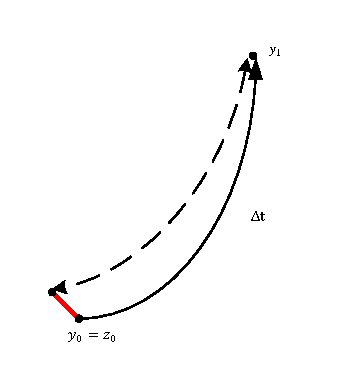
\includegraphics[width=.500\textwidth]{AtalenHasieraketa1}
}
\subfloat[Atalen hasieraketa2.]{
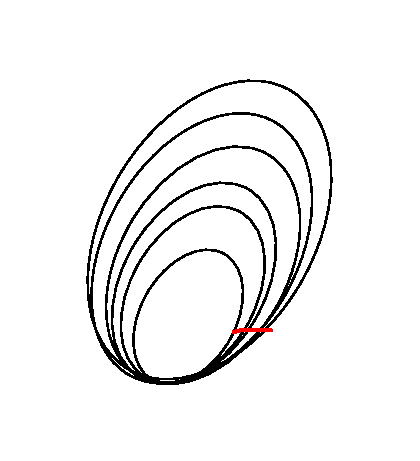
\includegraphics[width=.500\textwidth]{AtalenHasieraketa2}
}
\caption[Atalen hasieraketa.]
        {\small ....        
         \textbf{(a) irudian},                           
         \textbf{(b)} ......        
        }
\label{fig:Atalak12}
\end{figure}   

\begin{figure}[h]
\centerline{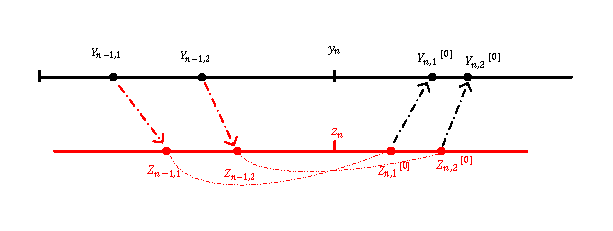
\includegraphics[width=12cm, height=6cm] {AtalenHasieraketa3}}
\caption{Atalen hasieraketa3.}
\label{fig:lau}
\end{figure} 

\section{Denbora birparametrizazioa.}

\subsection*{Sarrera.}

Uurrats luzera finkoa, ez da kolisio gertuko egoerak dituzten sistema dinamikoak edo denbora maila oso ezberdinak dituzten problemak integratzeko eraginkorra. Erregularizazio da arazo honen aurrean teknika arrakastatsuena. Erregularizazioaren bidez,  gorputzen arteko distantzia zerorantz hurbildu arren, mugimenduaren ekuazioak ez singularrak mantentzen dira.   

Demagun jatorrizko ekuazio diferentziala,
\begin{equation*}
\dot{y}=f(y(t)),
\end{equation*}

non $y$ menpeko aldagaia eta $t$ aldagai askea den.

\paragraph*{} Aldagai askeari aldaketa bat aplikatuz ($s()$ izeneko funtzio), ekuazio diferentziala leuntzea lortuko dugu. 

\begin{equation*}
y=z,
\end{equation*}

\begin{equation*}
\frac{dt}{d\tau}=s(z)
\end{equation*}

\paragraph*{} Honako garapena egingo dugu aldagai berriarekiko ($\tau$) ekuazioak lortzeko.

\begin{equation*}
y=z \ \ \Rightarrow \ \ \frac{dy}{dt}=\frac{dz}{d \tau} \ \frac{d \tau}{dt} \ \Rightarrow \ \frac{dz}{d \tau}= s(z) \ f(y(t)) 
\end{equation*}

\paragraph*{} Sistema berrian, mugimendua $z(\tau)$ funtzioak deskribatzen du: $z$ aldagai berria $\tau$ aldagai askearen menpekoa da. 

\subsection{Adibidea.}

Esperimentu honetan, IRK metodoan denbora birparametrizazioa modu errezean aplika daitekeela erakutsi nahi dugu. N9-Body probleman, merkurio ezentrizitate handiena duen planeta da: merkurio araberako denbora birparametrizazioa planteatuko dugu.

\begin{equation}
s(q)=r_{10}^{3/2}
\end{equation}

\begin{equation}
r_{10}=\|q1-q0\|_2
\end{equation}

non $q_1=(q1_{x},q1_{y},q1_{z})$ merkurio plantearen kokapena eta $q_0=(q0_{x},q0_{y},q0_{z})$ eguzkiaren kokapena den.

\section{Laburpena.}